\documentclass[a4paper]{article}

\usepackage{geometry}
 \geometry{
 a4paper,
 total={120mm, 257mm},
 left=20mm,
 top=20mm,
 }

\usepackage{titlesec}
\usepackage{graphicx}
\newcommand{\sectionbreak}{\clearpage}
\renewcommand{\figurename}

\usepackage{times}
\usepackage{hyperref}

\usepackage{marginnote}
\setlength{\marginparwidth}{5cm}
\setlength{\marginparsep}{1cm}


\usepackage{lingmacros}
\usepackage [document]{ragged2e}
\usepackage{booktabs}

\usepackage{graphicx, float}
\graphicspath{{pics /}}

\begin{document}
\section*{HIGH SCHOOL \\ARTISTIC INDUSTRY IN PRAGUE}
\thispagestyle{empty}
Bachelor Thesis \\
\vfill
2019 \\
Jan Šindler

\section*{HIGH SCHOOL \\ARTISTIC INDUSTRY IN PRAGUE}
\thispagestyle{empty}
Font and Typography \\
Bachelor Thesis \\
Jan Sindler \\
\vspace{20mm}
Digital Imaging Font \\
\vfill
Prague, 2019 \\
Thesis supervisor: Tomáš Brousil \\
Bachelor Thesis Consultant: Lukáš Pilka \\

\section*{ACADEMY OF ARTS, \\
ARCHITECTURE AND DESIGN IN PRAGUE}
\thispagestyle{empty}
Typography and Typeface Designing \\
Bachelor thesis \\
Jan Sindler \\
\vspace{20mm}
Typeface for digital displaying \\
\vfill
Prague, 2019 \\
Bachelor Thesis Supervisor: Tomáš Brousil \\
Bachelor Thesis Consultant: Lukáš Pilka \\

\section{introduction}
\setcounter{page}{1}
I chose the theme mainly due to the influence of the internship at LucasFonts in the summer of 2018. I learned a lot at the internship and found that our practice is not just about shaping curves. LucasFonts is dedicated to designing and producing the finest fonts that will last for years. I was happy to be part of the team and I hope to be back again. For the first time when I heard from Lucas the magic words like VTT and hinting, I could only pretend to know what was being said. The first hinting experiments were already on the internship, it was mainly an attempt and error to apply the hinting method, I didn't get much of it. After the internship I started to work in fields like programming and I was interested in the structure of the font file. Hinting is still inherently part of the writing production and it is a pity that not many people already know about this craft. It is important to know its strength so that we can better design and satisfy not only our insatiable desire but also the end consumer. I want to have a deeper understanding of hinting so that I can do better typefaces, know the circumstances, and gain an advantage. During my studies, I lived in a naive idea of  the dominance of morphology over all other sectors of typeface design, and it is no longer my bachelor thesis and I move the morphology given by bezier curves even further. I will process the font, which will be based on the data I present in my bachelor thesis. I am mainly interested in the relationship of bitmap rasterized contour and contour itself. When it happens that our beloved typeface loses everything we have given it and is a few pixels? Can I suggest a font based on the grid constraint that is designed and not looking like from the 1990s? I want to make a font for 1-bit displays because I see hinting as a huge potential for these systems. I want to design an alternative to the best Verdana, which will offer a slightly different view of the subject and be as well worked out. I went to the design itself with great expectations about the discovery of the undiscovered, the reality and the sense of typography changed my direction and opinion a bit. The theoretical work itself deals with the analysis of the situation in the world of digital fonts and the overview of the so-called big data that I collected and analyzed. The results of the analyzes are the facts on which I base my project.

\section{What is hinting?}

Hinting, or screen optimization, is the process by which TrueType or PostScript fonts are customized to maximize display readability (Petr Biľak, typotheque.com/articles/hinting) Hint is a hinting guide, hinting is a kind of advice for rasterizer that is stupid and without the advice would not display the font well. There are 4 types of Beat Stamm, rastertragedy.com/RTRCh2.htm

\begin{figure} [H]
  
\includegraphics [width =\linewidth]{pics/o_1bit.png}
  \caption{full pixel - pixels are either on or off, 1 bit principle.}
\end{figure}

\begin{figure} [H]
  
\includegraphics [width =\linewidth]{pics/1bit_fullanti.png}
  \caption{full-pixel with full pixel smoothing - Full pixels are complemented by grayscale pixels that optically fill pixel teeth in the pixel distribution of full pixel rastering.}
\end{figure}

\begin{figure} [H]
  
\includegraphics [width =\linewidth]{pics/o_TT.png}
  \caption{asymmetric with non-pixel-smoothing - Pixel is horizontally composed of 3 sub-pixels, RGB - red, green, and blue. These shining sub-pixels vary in intensity according to complex algorithms based on optics and physics. Together with distance, they form a whole where we only see black and white. }
\end{figure}

\begin{figure} [H]
  
\includegraphics [width =\linewidth]{pics/o_TT_antialiasing.png}
  \caption{Hybrid - acts like the previous method in the X-axis. The Y-axis behaves similarly to the second way of rasterization, but it also works with the pixel colors themselves}
\end{figure}

\begin{figure} [H]
  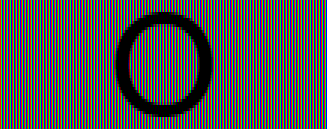
\includegraphics [width =\linewidth]{pics/o_TT_antialiasing_preview.png}
  \caption{Preview of how hybrid rasterization actually looks on the RGB LCD screen. RGB is the color order in one pixel, there are also BGR monitors.}
\end{figure}

\subsection{Hinting History}
Hinting is the programming language itself, before the advent of visual hinting, the curves had to be programmed in the way we usually imagine programming. However, with the advent of visual hinting, this method of text programming has not completely disappeared and some engineers still use it. But the visual style eased the craft mainly to our designers, who are not just focused on hinting and we are also engaged in other typography disciplines. (I should get some more info here)

\subsection{Hinting today}

Hinting is probably a dying craft today, designers are not interested in this font quality because they are working on high-resolution devices and they are unable to see the deficiencies themselves on their device. However, poor hinting will only be felt at the end user. It has to be admitted that hinting is not as necessary as it was previously used on desktop computers 20 years ago, the greater part of the devices will display the font well even without it. Yet even with a relatively modern computer, I still notice poorly crafted fonts on the web, which often make reading on digital devices very difficult, I'm talking about sites like the BBC and YouTube, which are definitely not peripheral issues. There are professions where people spend several hours a day at the computer, and they care about their readability. For example, an open-source Fira font is widely used by programmers. Users notice the wrong hinting, and although they often don't know how to name this problem, the font creators will report it to fix it. Do we not have the illusion that hinting cares no one, where did this mood actually come from, when we do such a typeface for printing?


\subsection{Types of Hinting}

\begin{enumerate}
\item \textbf{TrueType hinting}
is a very powerful tool that allows you to modify the letters of each size to the smallest detail, as a point shift for a certain font size even by 1/16 of a pixel. The tool is powerful and its control is very complex. TT hinting as we know it today can be imagined as a visual programming where we set rules. It is important to realize that it is a programming language and each character has a program in such a language assigned to it, which communicates with the rasterizer and advises him how to render, then it is on the rasterizer itself to deal with such advice.

\item \textbf{PostScript hinting}
PostScript hinting is a more modern form of hinting, it is simpler than TrueType but does not allow such modifications.

\item \textbf{Autohinting}
It is automatic to create a hinting program for font characters. TrueType can work either on PostScript hinting and good font settings (it will work more accurately than if the algorithm attempts to automate hinting without them). TT autohinting can come across when it is a nonstandard font, for example, when the end of stroke are not placed directly on the baseline. Also, we cannot apply autohinting to fonts where awareness of font context is important. I have already felt this when working on variable fonts where I could only hint in the Y-axis. That wouldn't be a problem yet, all the characters were in groups, and they had to be the same as the children of this group.

\begin{figure} [H]
  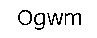
\includegraphics [width =\linewidth]{pics/no_hinting.png}
  \caption{Sample text without applying hinting at 1-bit rasterization. A tiny difference in points will result in unwanted rounding. Typically, the letters have different stroke thicknesses}
\end{figure}

\begin{figure} [H]
  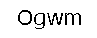
\includegraphics [width =\linewidth]{pics/autohinting.png}
  \caption{Autohinting did a little better. It can be seen that the algorithm has no notion of symmetry and context in typography. The horizontal stroke of 'O' is a pixel thicker because the contour is also a few points thicker, but this is needed for optical compensation for printed typography. The stroke thickness is set larger so that the characters are optically the same dark. Specifically, in this case, the stroke thickness is 42 points for the capitals and 40 for the mines, the distance of 42 points for that size is already rounded to 2 pixels, however, the distance of 40 points is still rounded to 1 pixel. Up to 255 and more should have such optical compensation, because just in size 255 the horizontal stroke of the capitals starts with 21 pixels, in the case of minuses it can be 20. Every 21 pixels in addition to the horizontal stroke of the capitals can add 1 pixel in addition to the difference between by this stroke in caps and mines. In addition, it is hard to guess what the algorithm was chasing when it applied compensation to the round stroke connection to the stroke at 'm'. }
\end{figure}
\end{enumerate}

\section{hinting programs}
Hinting can be done directly in the font editor or in an external editor. The implemented editor has the disadvantage that it is not as specialized and powerful as the external one. On the other hand, the production of such a font with the implemented hinting editor is easier because all the data is in one place and there can be no problems changing the order of the points in the contour.

\subsection{VTT}
VTT is the most powerful and professional hinting editor that exists. It is developed by Microsoft and they also produce fonts. I will briefly present the basic tools that VTT  has and many other editors also often have.
\begin{enumerate}
\item Link - the basic tool for determining which one point relationship fits to another. These can be simple rules - rounded to the left, rounded to the other to the left, or that the two 'a' and 'b' points are the same number of pixels apart as the other two 'x' and 'y' points.

\item Interpolate - interpolates one point based on the other two - something like placing a sticker on the spring and then stretching the spring, the point will always be in the same distance to the edges of the spring.

\item Delta - Scroll either local or global values  - if we set all points on x-height \marginpar{X-height, x-height in Czech also middle puncture, is height main masses of minus signs, leading just where the lowercase 'x' ends} are represented by the same variable, the delta can be used to determine in which sizes the height of a point is raised, if we are not satisfied with the smoothness of the gradation. The local delta then controls points in the same way, from the finest nuance of 1/16 point to 8 points plus and minus, if there is any reason, we can set the letter 'o' to be wider or narrower by up to 8 points in selected size. Such a modification does not make sense, but nicely demonstrates the power of VTT.

\end{enumerate}

\subsection{rasterizers}

rasterize - Convert an image stored as a curve to a pixel image that can be displayed on a digital device or printed. (en.oxforddictionaries.com/definition/rasterize). An image written by curves is mathematically written a shape, so that shape is infinitely magnifiable. Although it does not seem so to us, printers also need to rasterize all the curves we want to print on them. It is a conversion from a mathematically written form to data that can be stored either in a two-dimensional or three-dimensional matrix. Three-dimensional if one cell contains more than one value. Thus, a color image itself is a three-dimensional matrix.
\marginpar{
A matrix is a mathematical rectangular or square diagram of numbers or some mathematical objects - elements of a matrix (also matrix elements). (cs.wikipedia.org/wiki/Matice)
}

\begin{enumerate}
\item ClearType - Windows rasterizer, based on pixel-to-sub-pixel division. RGB = 1 pixel, R = 1/3 pixel ...

\item FreeType - an open source project found in a large number of devices. From Android/Linux to Apple phones. This is an open source variant of ClearType. FreeType includes up to a billion devices in the world (freetype.org).

\item Quartz - rasterizer MacOs, it ignores all hinting instructions and creates the raster according to its own algorithm, so that the text appears on the screen as much as its printed form. As a result, the fonts are very poorly readable in small sizes.

\item CoolType - is a method of text rasterization used by Adobe and its many programs
\end{enumerate}

\section{analysis}
Therefore, to better understand the data around the fonts and the digital footprint they leave in the world, I used Google's services called BigQuerry. It allows you to search huge amounts of data in seconds. BigQuery \marginpar{
bigquery.cloud.google.com}
moreover, it offers its own datasets for free. I mainly used the dataset \marginpar{
Dataset is a data file that is free for BigQuery. It can go as
} by github, I was mainly interested in what proportion of serif and non-serif fonts are used on the web and also what font size is most used.

\subsection{font-size}
Today's computer screens in most of the world have almost no problem with displaying text, but we must not forget the areas or institutions where it is very difficult to switch to a newer system, either because of its own internal tools that are very difficult to update or because of lack of finance. Large companies should have a font that can withstand any situation, even on the weakest device or in an application where even tiles and paving stones are pixels themselves. A typical example is a washing machine display, a boiler display, a digital price tag in the supermarket, the power-on monitor's start-up screen, or when setting it in the menu, as well as any other simple computer system that does not support state-of-the-art imaging technology. We must not forget the still relatively strong user base that still works on Windows XP by 2017 data, these users should be more than Linux users or MacOs Sierra (businessinsider.com/how-many-people-use-windows-xp -chart-2017-5). Windows Xp allows the additional installation of a ClearType raster engine, but it is very likely that only a small portion of these computers will be dipsonated. All these devices require either application of corporate fonts, logos or pictograms. Here everywhere hinting fits. I designed the font primarily for yet unknown size, which is the most widely used by people, I only entered my request for setting up the website, mainly because it is fixed and the programmers choose the size, knowing that they do not know what device their website will display and I assume that the design habits for a single platform, they can also be seen when designing on a second platform. Since this is an academic task, I do not know what device my font will be displayed on. The more interesting it is because I want it to look, read and work well on all facilities and in many circumstances. For my analysis, I used the BigQuery service, which allows you to explore large amounts of data using their own computers. Google has already provided us with some data in this service, a dataset called such a data package. We can imagine such a dataset as a very large Excel table that is so big that we wouldn't open it on our computer, probably stuck and wouldn't even be halfway. One of the datasets is GitHub data \marginpar{
GitHub is a developer platform where people can store and share an application being developed, either with each other or with the public.
} has 2.3TB \marginpar{TB as Terabyte, GB as Gigabyte are units for describing the size of digital data}, I only made my attempt on the unpaid 30GB and even so I got satisfying results that are sufficient for quantity . The analysis showed that programmers use PX units to a large extent over PT. So the full dataset is 2.3TB, that's 80 times more than the dataset I used. I don't want to convert terabytes to film hours, but I would say that 2.3TB is the memory capacity of 5-7 notebooks in 2019. The PT font unit is designed for printed output, so programmers are aware of the specifics of digital fonts. The data showed that the most used size for websites is 14PX and 10PT, which equals 13.3PX. Thus, the basic size for designing a digital imaging font is 14PX. This is the size where differences between hinting unibody fonts are just beginning to break and fonts are already beginning to differ. The B/W grid of the monitor is limited and therefore some fonts may look similar, even though they are either egyptian and serif fonts. In the case of small sizes, however, it cannot be different but guarantee that the font will work in small sizes. Not to mention the adaptation of the pictograms and logos to such views.

\begin{tabular}{r | rrr}
unit & \\
& median & \\
& & m. average & \\
& & & find count \\
\midrule
PX & 14.0 & 26.8330 & 13352 \\
PT & 10.0 (13.3330PX) & 12.3086 & 1231 \\
EM & 1.2 & 3.0410 & 7225 \\
\% & 100.0 & 114.9932 & 6295 \\
\end{tabular}

\subsection{font-family}
My next goal of exploring with BigQuery was what fonts programmers use. The results show that fonts are sans-serif and mostly system preinstalled. It follows that programmers are aware of the benefits of such fonts. However, the system may not display system font on another platform because they are not present on the system. Sans-serif are generally more readable on screens of lower resolution, they are free of details that the screens are unable to display. Among these twenty most used fonts is only one serif, it is very surprising that Times New Roman didnt get into this twenty. Whether the absence of serif fonts is a consequence of a weak supply or, in digital design does not seek such fonts, is for discussion. Fonts are set for websites either specifically or as a group, ie font name - Arial - or font type - Sans Serif. On each system, the Sans Serif group is then defined in a different font, on Windows it is probably Arial while on Mac it is Helvetica. The font does not have to be set to only one, but if the font on the target device is not, it would be replaced by an uncontrollable basic font of the platform. For example, if we plant the web in Helvetica, Windows will display this font in Times New Roman, because there is no Helvetica there. We do not want to do this, so we can set the fonts to your preference in the order of our preferences, unless the first one is in the system, the next one is applied, and so on.

\begin{tabular}{r | rlr}
font/group name & \\
& Finds & \\
&& distribution & \\
\midrule
sans-serif & 25895 & Group \\
Arial & 20070 & WIN \\
Helvetica & 11886 & MAC \\
Helvetica neue & 6560 & MAC \\
Verdana & 5618 & WIN \\
monospace & 4881 & Group \\
Courier & 4315 & WIN \\
Tahoma & 2953 & WIN \\
inherit & 2943 & Group \\
Lucida console & 2239 & WIN \\
Font Awesome & 2163 & ID \\
serif & 2146 & Group \\
Lucida grande & 1733 & OS X \\
Monaco & 1413 & OS X \\
Lato & 1191 & G \\
Open sans & 1135 & G \\
Courier new & 1119 & WIN \\
Consolas & 1099 & WIN \\
Georgia & 1038 & WIN \& MAC \\
Segoe ui & 819 & WIN \\
\end{tabular}

\section{Pixel and pixel outside the digital world}
Rasterization must not be strictly understood as something that occurs solely on screens and, on the eye, on a non-traceable scale when printing, it is the distribution of curves on a regular grid. The regular and controllable distribution of raster curve points is especially important when the grid density is reduced or increased. Here are three examples where this distribution is also useful for applications other than the screen. All these applications are very likely, and if a company has a hinted font once, the problem of rasterization anywhere will never have to be solved. \\

\begin{enumerate}
\item \textbf{Needle printers} with the obligation to print all receipts in the Czech Republic, the consumption of thermo paper is growing, but it is not recyclable and environmentalists often point out this fact. Shops familiar with this issue use old dot matrix printers because they are recycled and recyclable paper. It is a trend that spreads across bio-shops and cafes, but it solves the problem of non-recyclable thermo papers and shows us that no technology is dead and there is a good chance it will come back soon or later.

\item \textbf{Pixel Work}
The digital raster image is not just a sequence of shapes and points but an accurate grid with accurate data, which we can use today and work with the pixels themselves. It is not at all difficult as a designer to create a tool that transforms a pixel into another shape. Such a tool will then be created for example by the festival visual by simply applying the instrument to the photograph. Just van Rossum and Hansje van Halem showed us great in visuals at the visual styles of the Lowlands and the Norm studio when designing a new look for Swiss banknotes. If I have a 2x2 pixel chessboard array, the image data would look like this [[255, 0], [0, 255]]. We can then work with the data at will. For example, we can include all of the fields where white (255) links them with a line or replace them with a symbol. We can replace them with faces or hearts, the net would then be much larger than we would expect from a 2x2 pixel image. This image now becomes a network where each point can be observed separately. However, together they form a whole where even distribution is important.

\begin{figure} [H]
  \includegraphics [width =\linewidth]{pics/pixels.png}
  \caption{individual pixels are represented behind the graphic elements}
\end{figure}

\item \textbf{Design Production}
There are technologies where the detail is very limited in design implementation. Typically, it can be knitting, weaving, embroidery, or perforation in a variety of materials, or even putting the inscription into tiles, tiles, or roof tiles like the St. Stephen's Cathedral in Vienna.
\end{enumerate}

\subsection{Times' text is the same as Arial}
The unique shape of the letter we are accustomed to judging from paper, and we are so proud of as typographers, transforms into screens and is something we have never wanted. In the smallest sizes, our fabrications disappear, the typeface is unreadable, and we are angry. Hinting guarantees legibility even in the smallest sizes. With a grid smaller than 20 points, the finest details disappear and one font starts to remind the other. If anyone thinks that making a font is about making letters different from those before us, they're wrong. Whether the fonts are really identical are examined in the following experiment. I compare the bitmaps for arial.ttf, georgia.ttf, tahoma.ttf, verdana.ttf, consola.ttf, lucon.ttf, and times.ttf in 8, 9, 10, 11, and 12 pixels in single-bit delivery.\\
\vspace{20mm}
\begin{tabular}{r | cccccccccccc}
\rotatebox[origin=l]{90}{matches} &
\rotatebox[origin=l]{90}{same letter} &
\rotatebox[origin=l]{90}{font-size} & \\
\midrule
5 & o 9 & o 9 & o 9 & o 9 & o 9 & o & ti 10 \\
4 & O & A 9 & O & Ti 9 & O & Ti 10 & 0 & Lu 11 \\
4 & 8 & 9 & 8 & 9 & 8 & 9 & 8 & 10 \\
3 & i 8 & l & a 8 & i & a 8 \\
3 & D & A 8 & D & Ta 8 & D & Co 10 \\
3 & e 9 & e 9 & e 9 & e 9 \\
3 & t 9 & t & t 9 & t & t 10 \\
3 & j 9 & j & ti 9 & j & ti 10 \\
3 & l 9 & l & Ti 9 & l & Ti 10 \\
3 & u 9 & u & ti 9 & u 10 \\
3 & 0 & Ta 9 & 0 & Ti 9 & 0 & Ti 10 \\
3 & e & G 10 & e & Ta 10 & e & Ti 11 \\
3 & 0 & G 10 & o 10 & o & Ti 11 \\
3 & o 11 & o & ta 11 & o & ti 12 \\
\end{tabular}
\vspace{20mm} \\
A = Arial, G = Georgia, Ta = Tahoma, Ti = Times, Lu = Lucida Console, Co = Consolas \\

\section{Delta Design}
After all these surveys and understanding the issues, I could only start designing a contour. I see the potential for using this technology mainly in large companies, where it is not known where their font can appear. I want to offer an alternative to Verdana, which reflects today's visual culture and is equally well matched to one-bit displays. We are very limited in the search for fonts for such displays and we will most likely end up in Verdana most often. I went into this struggle with optimistic ideas to discover something undiscovered. But I soon realized the quality of Verdana, and I realized that the morphology she had could not leave so completely. Is it possible that Verdana is the last major digital imaging project?

\subsection{Consultation}
In the TypeDrawers forum \marginpar{typedrawers.com, there is a forum with a strong community where people advise on issues related to perhaps all typefaces} I came across a font engineer and designer - Mike Duggan, was very willing to consult with me and he explained to me the most basic principles that a person applies when hinting fonts. Mike works at Microsoft and has hinted for example Times New Roman. So he gave me a great enough insight into the issue of hinting and explained to me the problems faced by engineers in practice. Although the Internet seems to be endless, the resources from which I could learn in the VTT program are very limited. Mike is one of the few people in the world who have mastered this tool and was so willing to share his experience with me.

\subsection{Grid \& Contour In It}
When designing the contour itself, I wanted to draw on the constraints given by the most widely used grid, that is, the data show, with a 14px grid. Just the sizes around this one should be the most used ones. If we design fonts with constraints, there will be nothing to limit in small sizes. Hinting at that moment is not a limitation of the rich contour, but the contour gets into its natural environment. The constraints it determines should translate into the final contour form so that the original and functional contours do not lose their face in their bitmap version. I sketched in a squared block or drew straight on the computer in one-bit mode. I was hoping that in this way I would find the limitations that such grids offer. For the middle height I defined 8 points, the capitals are 2 points higher and the lower end points 2 points lower, the upper post is then one point higher than the capitals. 



Difference between mid-height and capitals by just 2 points is important for the primary size of 14px mainly because of contour identity across capitals and minuses in this size. He transferred the grid resolution to the font grid so that one grid grid has dimensions of 44 * 40. Thus, the vertical shaft has a thickness of 44 points and a horizontal stroke of 40. The font is designed for several pins, most often 4-6 points wide, with slight optical adjustments for printing. This is based on the fact that the letters in these pins end in 1-bit display, so why not suggest them directly?
\subsection {Safe Angles}
for even distribution of pixels on diagonals, the angle at which the diagonals are is very important. The diagonal angle in my font is one of the diagonal angles of the rectangle with an aspect ratio of 1: integer. For 1: 1 it is 45 degrees, for 1: 2 it is 26.5 etc. This shape then fills the contour, either rises one point to the right and up or one to the right and two up.
90,
45,
26.5 a
18.5 degrees are the most useful safe angles for the screen. In my writing, I try to adjust all the diagonals to these angles. There is a rather large difference between 45 and 26.5, and when the diagonal does not fall on either of these angles, I use an artificial safe angle, ie. for example, a rectangle angle of 1: x.5. But in very rare cases I was forced to drop the safe angle.

\begin{figure} [H]
  \includegraphics [width =\linewidth] {pics/safe-angles.png}
  \caption {Safe angles used in the font. There is a big gap between 90 and 45 degrees, and not every shape can fit into that angle. I had to extend the range of these angles with the so-called speudo-safe angles in a minimum number of characters. Which is the diagonal 1: x.5 of the square, most often 1: 0.5.}
\end{figure}

\begin{figure} [H]
  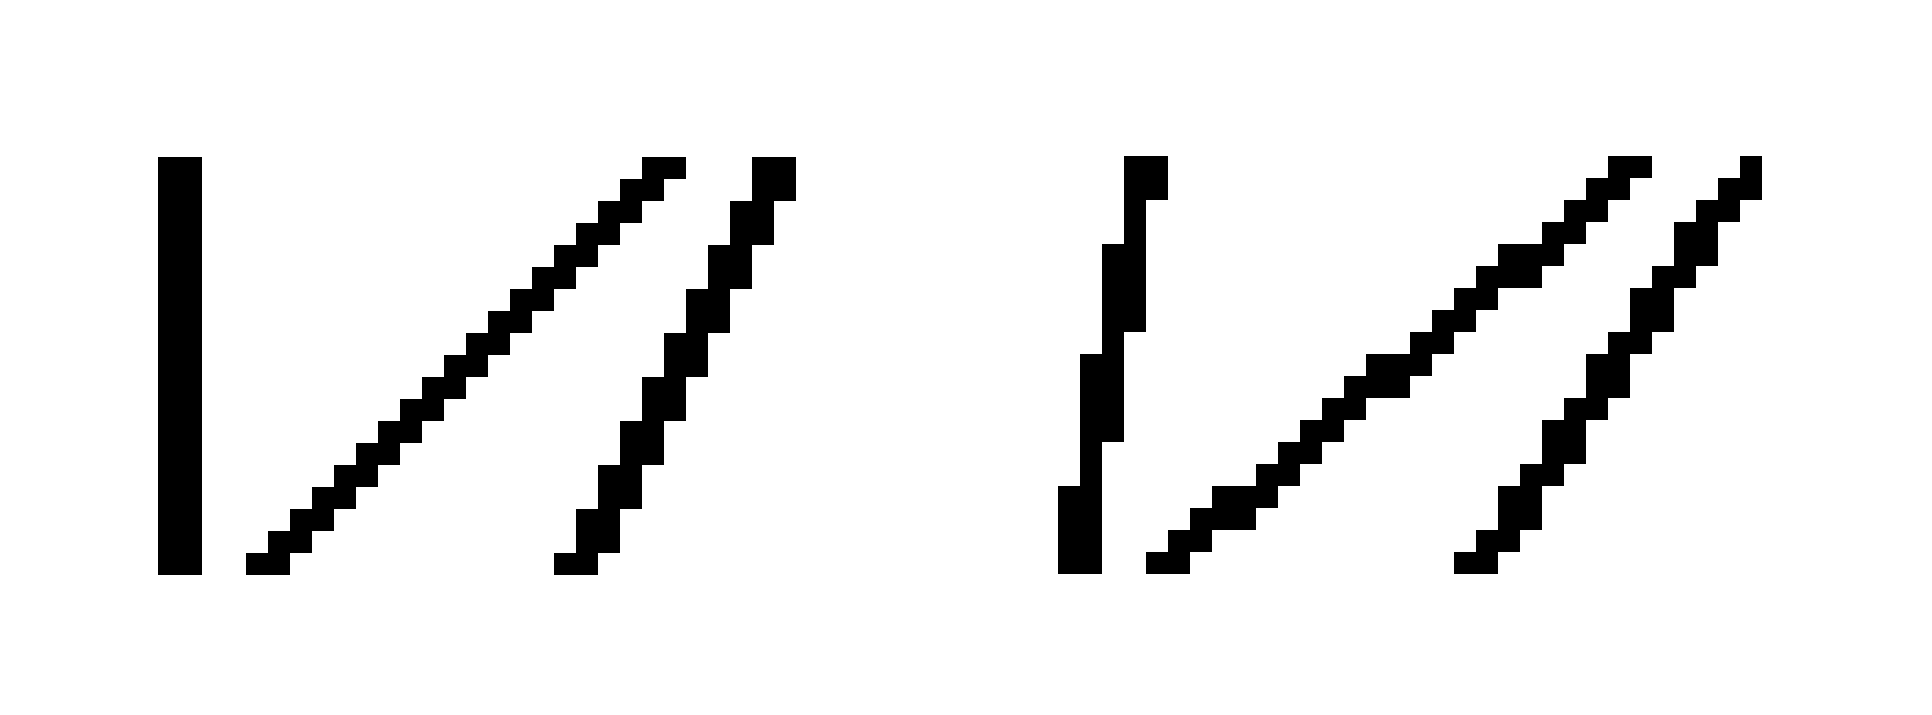
\includegraphics [width =\linewidth] {pics/1bit.png}
  \caption {three diagonals left at 90, 26.5 and 18.5 degrees on the left, but the same at 10 degrees to the right. One-bit rendering}
\end{figure}

\begin{figure} [H]
  \includegraphics [width =\linewidth] {pics/bw.png}
  \caption {same diagonals. Single-bit rendering, 14px size}
\end{figure}

\begin{figure} [H]
  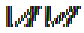
\includegraphics [width =\linewidth] {pics/truetype.png}
  \caption {Same diagonals, TrueType}
\end{figure}

\begin{figure} [H]
  
\includegraphics [width =\linewidth] {pics/truetype_bw.png}
  \caption {brightness intensity preview of pixels at TrueType rasterization}
\end{figure}

\begin{figure} [H]
  
\includegraphics [width =\linewidth] {pics/pseudo.png}
  \caption {90 degree move and strokes under pseudo-safe angles 33.7 and 21.8 degrees. Pixel distribution is not quite even as with safe angles, but a certain and still readable pattern is there.}
\end{figure}



\subsection{Contour}
The contour is the result of endless redrawing and exploration of contour behavior in hinting. As I have already mentioned, an important factor for 1-bit letters is the even pixel distribution, ideally at an angle of 45 degrees or under a different angle. Thus, the diagonal of the letters tries to keep the angle of 45 degrees best, or another of the safe angles. The contour does not need to strictly adhere to the grid from which it comes out, which would be detrimental to the other side of the printed use. There are few moments in my font that are really handy while hinting. It can be an extra point that would normally be considered a bug, but is useful for hinting because we can interpolate from it, for example. This approach is more visible, for example, with the letter 'x', where I emphasize a verical stem that often appears in small bitmap font sizes. This element also helps a lot of hinting itself. The potential digital use of the font can be primary but certainly not the only one in the case of my work, so it is important to think that the font is good and original in every application. Thus, fonts must meet the qualities that require print media and digital use.
\subsection{Hinting}
Maintaining even pixel distribution is very demanding in 1-bit rendering, we can compare the images above this section by ourselves. The X-axis has three times higher resolution in the case of TrueTypes, which we cannot easily observe on the devices. It is important to remember that a pixel can be large in size and viewed from any distance, both in context and without context. Pixel division is not noticed on your computer monitor, but we notice it on a large LED installation that can be accessed from any distance? The aesthetics of the font is also influenced by the tools of the VTT hinting program. Setting an angle there is not straight, but the distance can be worked in several ways. If we know the distance of two sides of the triangle, we can set the diagonal angle with them. This way is limited only by two things. 1. is a clarity of working data, for each distance we have to store one variable in the distance drawer. If there are so many variables, it is likely that we will lose track of the variables. 2. the height of the triangle is limited by the still unknown variable - the height of the poles. Thus, for vertical movement, a free space is needed to stretch the vertical side of the triangle. Simply put - the height of the diagonal stretched from baseline to height x is given by the height x, so we cannot set it by absolute value. Hinting for the smallest sizes came to me like creating contoured cartoons. The lowercase letters cannot be perceived in the same way as the uppercase ones, and it is sometimes necessary to overdo a bit, to pinpoint a characteristic element and to help readability more than at large print sizes.
\subsection{Slideshow}
I tested my font on Nokia 5110 displays during the process. This 5110 is now sold as an open module and is ready to get into it. At the same time, it is a representative of the one-bit displays I focus on, and that is why it was a clear choice for presenting and testing my Delta font. As a computer for rendering letters I use Raspberry Pi Zero WH, which runs a program written in Python 3 that uses the FreeType library as a rasterizer, so the result is identical to how the font would behave on a Linux-based device. Testing the font on this rasterizer is a good good choice, mainly because there is a great possibility that the final use of the font will be on the device with this rasterizer. I also use Python for graphical outputs in this document and for other graphical outputs of my final presentation. For example, what is already mentioned is the substitution of pixels for graphical elements.
\subsection{Summary}


\end {document}